\documentclass[aspectratio=169]{beamer}

%%%%%%%%%%%%%%%%%%%%%%%%%%% 
%%%%%      TEMA      %%%%%%
%%%%%%%%%%%%%%%%%%%%%%%%%%%
\usetheme{Frankfurt}                      % theme
\usecolortheme{orchid}                    % colors
\usefonttheme[onlymath]{serif}            % font mathematical mode

%%%%%%%%%%%%%%%%%%%%%%%%%%% 
%%%%%    PACOTES      %%%%%
%%%%%%%%%%%%%%%%%%%%%%%%%%%

\usepackage[alf]{abntex2cite}             % citations in accordance with ABNT
\usepackage[brazil]{babel}                % language
\usepackage{color}                        % color control
\usepackage[T1]{fontenc}                  % source coding
\usepackage{graphicx}                     % figures
\usepackage[utf8]{inputenc}               % characters encoding
\usepackage{lmodern}
\usepackage{array}
\usepackage{multirow}
\usepackage{enumerate}                    % numerical indexes 
% \usepackage{footnote}                   % Handle footnotes
\usepackage{booktabs}                     % Tables with quality of publication in different situations
\usepackage{hyperref}                     % to cite web hyperlinks
\usepackage{adjustbox}
\usepackage{caption}
\newcommand\fnote[1]{\captionsetup{font=small}\caption*{#1}}

%%%%%%%%%%%%%%%%%%%%%%%%%%% 
%%%   INF. DOCUMENTO    %%%
%%%%%%%%%%%%%%%%%%%%%%%%%%%

% Titulo
\title[\sc{}]{How Big Data, Machine Learning and Text Mining can help predicting economic activity?}
\author{Hudson C. Costa, Sabino P. da Silva Júnior, Fernando A. B. Sabino da Silva}
\institute{Appus/HR Analytics, PPGE/UFRGS, Department of Statistics/UFRGS} 
\date{}


\usepackage{Sweave}
\begin{document}
\Sconcordance{concordance:apresentacao.tex:apresentacao.Rnw:%
1 41 1 1 0 634 1 1 3 1 0 1 4 2 0 1 4 7 0 1 4 135 1}



\begin{frame}
  \titlepage
\end{frame}

\begin{frame}[plain]\frametitle{Summary}
\small\tableofcontents
\end{frame}

\section{Introduction and Motivation}

\begin{frame}\frametitle{Introduction and Motivation}
  \begin{itemize}
  \item Economic Science has evolved over several decades toward a greater emphasis on empirical work. Hamermesh (2013) reviewed publications of the leading journals for the period 1963 to 2011:
    \begin{itemize}
      \item Until the mid-1980s, most articles were theoretical. After that the share of empirical articles rose more than 70\% 
      \item Most data are assembled or obtained by the authors or generated through controlled experiments 
    \end{itemize}
  \item Currently, there are a greater availability of data which may affect economic research
    \begin{itemize}
      \item Measurement of inflation and the labor market
       \item  Consumer behavior, productivity and \emph{job search}
    \end{itemize}
  \item \emph{Big Data} makes accessible statistical approaches (\emph{Classification Trees}, \emph{Regression Trees}, \emph{Random Forest}) and computational (\emph{Machine Learning} and \emph{Text Mining}) already commonly used in other fields of research;
  \end{itemize}
\end{frame}

\begin{frame}\frametitle{Introduction and Motivation}
  \begin{itemize}
  \item Main Goals:
    \begin{itemize}
    	\item Discuss computational natural
    	language processing (NLP) techniques
    	\item Investigate whether the
    	sentiment conveyed by Central Bank of Brazil (BCB) about the economy in their statements using \emph{Web Scraping} (the process of extracting text from a web page) and \emph{Text Mining} affects the short-term inflation 
    \end{itemize}
  \item Some Results and Conclusions:
    \begin{itemize}
      \item We create an algorithm that extracts all text from minutes of Copom (Monetary Policy Committee of the Central Bank of Brazil) from BCB website and transform the pdf format into textual format to create a corpus;
      \item We constructed a sentiment index for the monetary authority based on a dictionary of feelings (Inquider) maintained by Harvard
      University
      \item Our results confirm that such approach can contribute to the economic evaluation given that the time series of the index seems to be related to important macroeconomic variables
    \end{itemize}
  \end{itemize}
\end{frame}

%%%
% Methodology
%%%

\section{Methodology}

\begin{frame}\frametitle{Methodology - Web Scraping}
  \begin{itemize}
  \item \emph{Web Scraping}:
    \begin{itemize}
      \item The information available on the Internet (\emph{Web}) is rearely in a suitable format to be extracted in an automatic and efficient way
      \item \emph{Web Scraping} makes easier the process of collecting such data;
      \item We design an algorithm to extract information from unstructured text:
      \begin{itemize}
        \item The web pages are constructed using HTML language (HTML)
        \item The codes have \emph{tags}, such as <title> and <p>;
        \item These \emph{tags} to remain constant over time while the information inside them (minutes of Copom, for example) is dynamic;
        \item The algorithm is taught to use such \emph{tags} to locate information and store it in a database
      \end{itemize}
    \end{itemize}
  \end{itemize}
\end{frame}

\begin{frame}[fragile]\frametitle{Methodology - Web Scraping} 
  \begin{block}{Example of the minutes collection algorithm}
\begin{Schunk}
\begin{Sinput}
> main.page = read_html(x = "http://www.bcb.gov.br/?MINUTES")
> urls = main.page %>% 
+   html_nodes("#cronoAno a") %>%  
+   html_attr("href")  
> ano = main.page %>% 
+   html_nodes("#cronoAno a") %>% 
+   html_text() 
> 
> # 2016 http://www.bcb.gov.br/?id=MINUTES&ano=2016                                               
\end{Sinput}
\end{Schunk}
  \end{block}
  \begin{itemize}
    \item We have developed a system that carries out massive collection and then uploads the information to a database, based on a logical and scalable architecture solution
    \item It interacts with the web pages, extracts the information and stores the data
    \item Data Collectors: Google, Facebook.
  \end{itemize}
\end{frame}

\begin{frame}\frametitle{Methodology - Web Scraping}
  \begin{figure}[hb]
  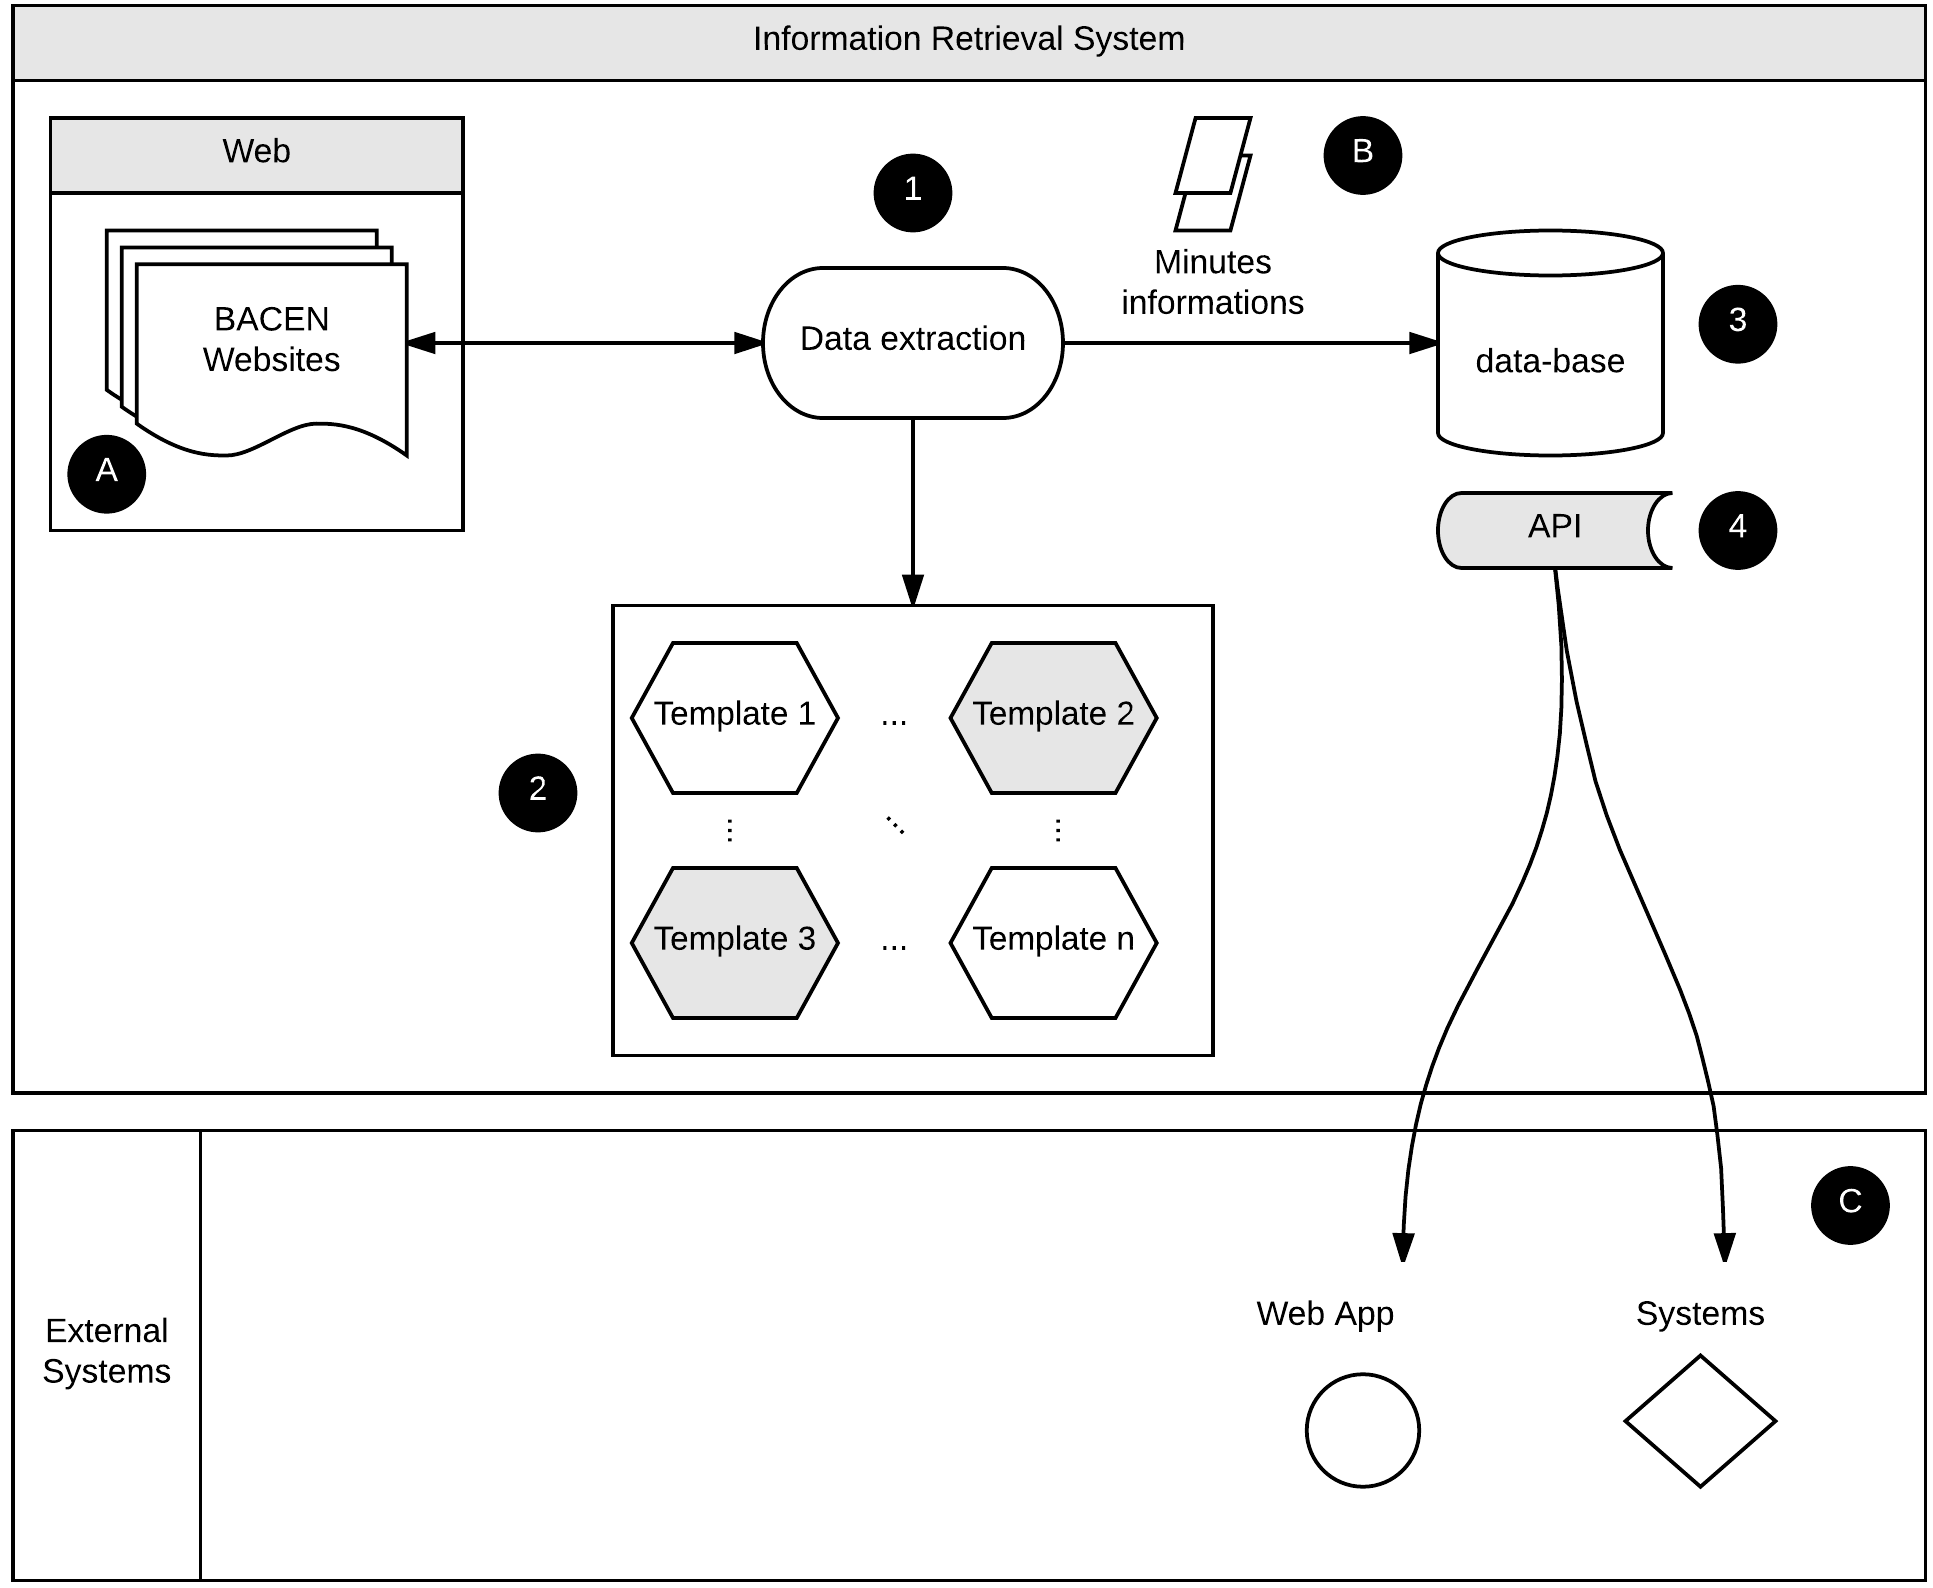
\includegraphics[width=3in]{minutes_crawler_diagram.png}
  \label{fig01}
  \end{figure}
\end{frame}

\begin{frame}\frametitle{Methodology - Sentiment Analysis}
  \begin{itemize}
  	\item It is the computational study of opinions, attitudes and emotions behind a series of words expressed within an online mention;
    \item The applications of sentiment analysis are broad and powerful. It allows us to gain an overview of the wider public opinion behind certain topics.;
    \item Two main approaches: (1) based on lexical resources and neutral language processing (it uses semantic dictionaries) and (2) employing machine learning algorithms;
    \item We follow the simpler approach of Hu and Liu (2004) and Kim and Hovy (2004), i.e., we focus in a dictionary-based approach for polarity identifications;
    \end{itemize}
\end{frame}

\begin{frame}\frametitle{Methodology - Sentiment Analysis}
\begin{itemize}
	\item When human readers approach a text, we use our understanding of the emotional intent of words to infer whether a section of text is positive or negative, or perhaps characterized by some other more nuanced emotion like surprise or disgust (Robinson and Silge, 2017).
	\item An often-used approach to analyze the sentiment of a text is to consider the text as a combination of its individual words and the sentiment content of the whole text as the sum of the sentiment content of the individual words. 
	\item We use lexicon that are based on unigrams, i.e., single words. 
\end{itemize}
\end{frame}

\begin{frame}\frametitle{Methodology - Sentiment Analysis}
\begin{itemize}
		\item The strategy is to first collect a small set of opinion words manually with known orientations, and then to grow this set by searching in an online dictionary for their synonyms and antonyms.
		\item The newly found words are added to the seed list. Then, the next iteration starts. It stops when no more words are found.
		\item We use the Inquirer dictionary provided by Harvard University (Stone, Dumphy and Smith (1966)) which classifies 11,788 words into semantic groups (\emph{positive}, \emph{negative}, \emph{strong}, \emph{weak}, among others).
\end{itemize}
\end{frame}

\begin{frame}\frametitle{Methodology - Sentiment Analysis}
  \begin{itemize}
    \item Using two databases (matrix of words of Copom minutes and semantic dictionary), we look for the words that are present in both bases for each of the minutes
    \item Thus, we know how many \textbf {negative} and \textbf {positive} words are present in each record of the minutes.
  \end{itemize}
  \begin{exampleblock}{Sentiment Index}
\[
{I}_{t} = \frac {{NP}_{t} - {NN}_{t}}{N} 
\]
  \end{exampleblock}
\noindent where ${I}_{t}$ is the sentiment index for each minute disclosed in $t$, ${NP}_{t}$ is the number of \textbf{positive} words present in the minutes reported in $t$ while ${NN}_{t}$ is the number of \textbf{negative} words and $N$ is the total number of words in the minutes. A higher value of the index ${I}_{t}$, signifies that the monetary authority has better expectations about the economyr.
\end{frame}

\begin{frame}\frametitle{Methodology - Data}
  \begin{itemize}
  	\item We use Copom's minutes to evaluate the BCB's sentiment about the economy;
    \item We use the English version available on the Internet and in PDF format since the 42nd Meeting;
    \item Total minutes available: 159 (until July 2016 meeting);
    \item We remove the minutes of meetings 42 and 43 from the sample due to differences in the layout of the files compared to the other minutes 
    \item In addition, using Quandl R package we collect the following time series to compare how well the sentiment index performs:
    \begin{itemize}
      \item Annual IPCA (National Consumer Price Index);
      \item Nominal interest rate (Selic);
      \item Annual inflation target
    \end{itemize}
  \end{itemize}
\end{frame}

%%%
% Results
%%%

\section{Results}

\begin{frame}\frametitle{Results}
  \begin{itemize}
    \item Once all minutes are stored, it is necessary to transform them so that each word can be extracted from its contents. 
    \item Next, we go through the following steps:
      \begin{enumerate}
        \item First we read and store PDF files in the format of a \textbf{Corpus} (a collection of textual documents);
        \item Here, our \textbf{Corpus} contains 157 textual documents, each document being a textual representation of the corresponding minute;
        \item Next, we format each text document to get rid from probable "impurities": 
        \begin{itemize}
          \item Remove numbers, punctuation characters, meaningless words (the, you, we, for example), blanks;
          \item Perform a word \emph{stemming} process, i.e., remove suffixes from words to get the common
          origin and transform all characters to lowercase.
        \end{itemize}
        \item Create a matrix where we have in each column the distinct words of all documents that belong to the \textbf{Corpus}. Each row represents a different document.
        \end{enumerate}
  \end{itemize}
\end{frame}

\begin{frame}\frametitle{Results}
  \begin{table}[h!]
  \centering
  \caption{Document-term matrix (Documents x Words)}
  \begin{tabular}{@{}lllllll@{}}
  \toprule
  Minute & absorption & acceleration & accommodative & accordance & according & account \\ 
  \midrule
  199th & 2.00 & 1.00 & 1.00 & 1.00 & 20.00 & 1.00 \\ 
  198th & 2.00 & 1.00 & 1.00 & 1.00 & 19.00 & 1.00 \\ 
  197th & 2.00 & 1.00 & 1.00 & 1.00 & 18.00 & 1.00 \\ 
  196th & 2.00 & 1.00 & 1.00 & 1.00 & 18.00 & 1.00 \\ 
  195th & 2.00 & 2.00 & 1.00 & 1.00 & 18.00 & 1.00 \\ 
  194th & 2.00 & 2.00 & 1.00 & 1.00 & 18.00 & 1.00 \\ 
  193rd & 2.00 & 2.00 & 1.00 & 1.00 & 23.00 & 1.00 \\ 
  192nd & 2.00 & 2.00 & 1.00 & 1.00 & 19.00 & 1.00 \\ 
  191st & 2.00 & 1.00 & 1.00 & 0.00 & 20.00 & 1.00 \\ 
  190th & 2.00 & 1.00 & 1.00 & 0.00 & 17.00 & 1.00 \\ 
  \bottomrule
  \end{tabular}
  \end{table}
\end{frame}

\begin{frame}\frametitle{Results}
  \begin{figure}[hb]
  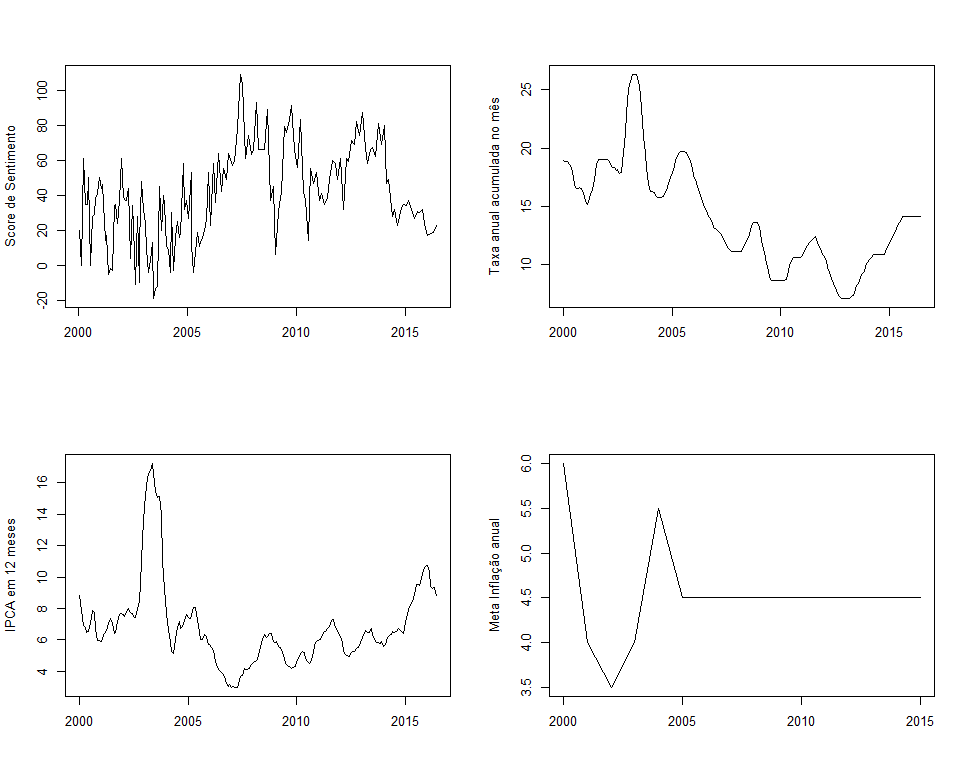
\includegraphics[width=3.5in]{comparative.png}
  \end{figure}
\end{frame}

%%%
% Conclusions
%%%

\section{Conclusions}

\begin{frame}\frametitle{Conclusions}
  \begin{itemize}
    \item We report an application of \emph{Text Mining} in the Copom minutes that are published on the BCB website;
    \item Using \emph{Web Scraping} and \emph{Text Mining} techniques we show that the sentiment index may help predicting economic activity. Thus, the arrival of economic information such as press-releases may be used to improve estimates of financial risk, for example;
%     \item To check the robustness of the results, we can conduct a Granger Causality test;
\item Future research will include econometric specifications augmented with news and sentiment indexes. We also will consider \emph{Machine Learning} techniques. 
  \end{itemize}
\end{frame}

\end{document}


% %%%%%%% REFERÊNCIAL BIBLIOGRÁFICO
% 
% \section{REFERÊNCIAS}
% \begin{frame}{Bibliography}
% \bibliographystyle{apalike}
% \bibliography{geral}
 
